%%%%%%%%%%%%%%%%%%%%%%%%%%%%%%%%%%%%%%%%%%%%%%%%%%%%%%%%%%%%%%%%%%%%%%%%%%%%%%
%
% Main content starts here
%
%%%%%%%%%%%%%%%%%%%%%%%%%%%%%%%%%%%%%%%%%%%%%%%%%%%%%%%%%%%%%%%%%%%%%%%%%%%%%%


\chapter{Introduction}
\label{sec:introduction}

This is a typical human-computer interaction thesis structure for an introduction which is structured in four paragraphs as follows:
% First Paragraph
% CORE MESSAGE OF THIS PARAGRAPH:
\todo{P1.1. What is the large scope of the problem?}
\todo{P1.2. What is the specific problem?}

% Second Paragraph
% CORE MESSAGE OF THIS PARAGRAPH:
\todo{P2.1. The second paragraph should be about what have others been doing}
\todo{P2.2. Why is the problem important? Why was this work carried out?}

% Third Paragraph
% CORE MESSAGE OF THIS PARAGRAPH:
\todo{P3.1. What have you done?}
\todo{P3.2. What is new about your work?}

% Fourth paragraph
% CORE MESSAGE OF THIS PARAGRAPH:
\todo{P4.1. What did you find out? What are the concrete results?}
\todo{P4.2. What are the implications? What does this mean for the bigger picture?}

LaTeX hints are provided in \autoref{chap:latexhints}.

\chapter{Background and related Work}
\section{Relevante Konzepte und Definitionen}
\subsection{Deepfakes}
"Deepfakes - Wenn man Augen und Ohren nicht mehr trauen kann" \cite{bildungDeepfakesWennMan2023} - So steigt Journalist und Autor der Bundeszentrale für politische Bildung Tim Walter in seinem Artikel über die Gefahren von Deepfakes ein. 
Dies ist nur eins von vielen Beispielen (Weitere Beispiele im Fußbereich) das zeigt, dass Deepfakes mittlerweile ein ernstgenommenes Thema in der nicht-technischen Medienwelt und Gesellschaft sind. 
Doch was genau sind eigentlich Deepfakes? 

\textcite{gambinDeepfakesCurrentFuture2024} beschreiben das Konzept Deepfake als "generation of fake digital content or manipulated of genuine one through the use of DL techniques." \cite[S. ?]{gambinDeepfakesCurrentFuture2024},
also frei übersetzt als die Erzeugung von gefälschten digitalen Inhalten oder die Manipulation echter Inhalte durch den Einsatz von Deep Learning Techniken. 
Deep Learning ist ein Teilgebiet der Künstlichen Intelligenz, genauer gesagt des Machine Learning, in dem es darum geht, mithilfe einer Reihe von Methoden automatisch Muster in Daten zu erkennen und diese zur Vorhersage zukünftiger Daten oder Entscheidungen zu verwenden \autocite[S. 1]{murphyMachineLearningProbabilistic2012} . 
Weiter schreiben Gambin et. al "The content inlcudes video, image, audio, and text among other sources." 
In einer ähnlichen Definition heißt es, dass bei Deepfake Videos in den meisten Fällen in einem schon existierenden Video das Abbild einer Person über den Körper einer anderen Person gelegt wird. 
Dadurch sieht es aus, als würde die Person dessen Abbild darüber gelegt wurde die Aktivitäten der anderen Person ausführen \autocite{harrisVideoDemandWhat2021}.
Währenddessen teilen \textcite{juefei-xuCounteringMaliciousDeepFakes2022} Deepfakes in die vier Kategorien "(i) entire face synthesis, (ii) attribute manipulation, (iii) identity swap, and (iv) expression swap (i.e., reenactment)". 
Schon an diesen Beispielen lässt sich erkennen, dass Deepfakes in unterschiedlichen Formen vorkommen.

Nachdem nun geklärt ist, was Deepfakes eigentlich sind, fehlt noch wo Deepfakes ihren Ursprung haben. 
Dazu schreiben \textcite{kernerPornDiscreditationEpistemic2021} "Deepfakes got started in 2017 [...] when an eponymous Reddit user enlisted open-source software from Google and elsewhere to apply scattered academic research to face-swapping". 
Die erste mediale Berichterstattung folgte im Dezember 2017 durch den Artikel \textcite{AIAssistedFakePorn2017} im Vice Tech Magazin Motherboard von Samantha Cole.
Seitdem nimmt die Verbreitung von Deepfakes immer weiter zu, was man unter anderem bei \textcite{ranaDeepfakeDetectionSystematic2022,westerlundEmergenceDeepfakeTechnology2019,gamagePDFEmergenceDeepfakes} sieht. 
Auch die Google Suchtrends zum Keyword "Deepfake" bestätigen diese Aussage, siehe Grafik \ref{fig:suchtrend-grafik}.
\begin{figure} [htbp]
    \centering
    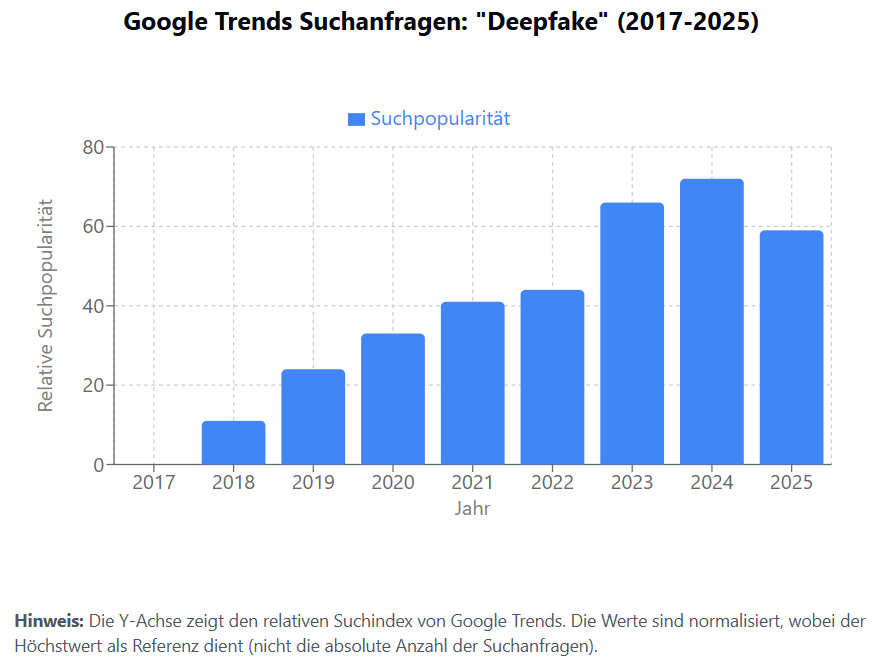
\includegraphics[width=0.8\textwidth]{GrafikGoogleTrendDeepfake.png}
    \caption{Google Suchtrend zum Keyword "Deepfake"}
    \label{fig:suchtrend-grafik}
\end{figure}

Seitdem werden Deepfakes allerdings auch immer wieder für negative Zwecke eingesetzt. 
Ein großer Einsatzbereich und auch der Ursprung von Deepfakes ist die Pornographie \autocite{ajderDeeptraceLabReport}. 
Aber auch abseits von Pornographie gibt es noch mehr kriminelle oder bösartige Einsatzbereiche von Deepfakes. 
Darunter sind unter anderem "spreading misinformation, creating political instability, or various cybercrimes" \cite{ranaDeepfakeDetectionSystematic2022} 
oder wie \textcite{gambinDeepfakesCurrentFuture2024} die Konsequenzen von Deepfakes als "far reaching, including the potential to ignite political or religous tensions between nations, decieve the public, disrupt financial markets, perpetrate acts of sabotage, fraud, scams, obstruct justice, and much more" beschreiben.
Im Folgenden einige Beispiele aus der Praxis von Fällen in denen Deepfakes mit krimineller oder bösartiger Absicht eingesetzt wurden.
\begin{itemize}
    \item Manipulation in der Politik: Ein Audio-Deepfake in dem der slowakische Spitzenkandidat Michal Šimečka scheinbar mit einer Journalistin über das Kaufen von Wählerstimmen diskutiert, 
        wird kurz vor der Parlamentswahl im Oktober 2023 veröffentlicht. 
        Dieser Deepfake wurde strategisch kurz vor der Wahl platziert und durch die slowakische Regelung, dass 48 Stunden vor der Wahl in den Medien kein Wahlkampf mehr betrieben werden darf, wurde eine Richtigstellung noch erschwert. \autocite{pawelecPolitischeManipulationUnd2024}
    \item Revenge Porn und andere nicht-einvernehmliche Inhalte: 
        Im Fall von Hannah Grundy wurden Deepfake Fotos mit pornographischen Inhalten von ihr auf einer Website "The destruction of Hannah" hochgeladen \autocite{WomansDeepfakeBetrayal2025}.
        In einem anderen Fall wurde im türkischen Wahlkampf ein Deepfake Video mit pornographischem Inhalt von Kandidat Muharrem İnce veröffentlicht, 
        was dessen Rücktritt aus dem Wahlkampf zur Konsequenz hatte. Quelle???
    \item Rufschädigung durch Nachahmung: Prominente wie Taylor Swift, Tom Hanks, Sabrina Carpenter und viele mehr werden regelmäßig Opfer von Deepfakes, die ihren Ruf schädigen sollen oder Produkte in ihrem Namen ohne ihre Zustimmung bewerben (Fox News 10 celebs most targeted by malicious deepfake scams, dangerous search results).
\end{itemize}
Bei all den negativen Beispielen ist zu beachten, dass die Deepfake Technologie an sich neutral ist und auch vielfache Weise positiv eingesetzt werden kann. Im Folgenden einige positive Beispiele wie Deepfakes eingesetzt werden können:
\begin{itemize}
    \item Filmindustrie: Erzeugen von Stimme von Schauspielern die ihre Stimme möglicherweise wegen Krankheit verloren haben. 2019 hat eine Malaria Kampagne David Beckham durch Deepfake Technologie multilingual wirken lassen um möglichst viele Menschen ansprechen zu können.
    \item Medizinischer Bereich: Durch Deepfakes können Alzheimer Patienten mit jüngeren Gesichtern, die sie möglicherweise wiedererkennen, interagieren. 
    \item Wirtschaftsbereich: Das digitale Anprobieren von Kleidung kann durch Deepfake Technologie ermöglicht werden.
\end{itemize}
(Westerlund 2019)

Diese Beispiele zeigen, dass die Deepfake Technologie jetzt schon in der Gesellschaft verankert ist, und sich in Zukunft noch weiter ausbreiten wird.
\chapter{Study Design}

\gls{er}

\section{Apparatus}

\section{Procedure}

\section{Measurements}

\section{Participants}

\chapter{Results}

Lorem ipsum dolor sit amet, consectetur adipiscing elit. In at nunc ut ex aliquam fermentum nec ut orci. Pellentesque habitant morbi tristique senectus et netus et malesuada fames ac turpis egestas. Vivamus sollicitudin pulvinar est, quis porttitor nisi egestas id. Cras et dignissim elit, vitae fringilla arcu. Aliquam rhoncus convallis aliquam. Aliquam erat volutpat. Proin efficitur sapien et velit aliquet imperdiet. Aenean tristique augue ultricies enim venenatis, ut mattis massa fringilla. Vestibulum ante ipsum primis in faucibus orci luctus et ultrices posuere cubilia curae; Duis vitae lobortis nunc. Nulla facilisis leo sed gravida elementum. Integer suscipit scelerisque lacinia. Nulla consectetur maximus purus a varius. Curabitur porta orci nisi, non porttitor lectus hendrerit vitae. Nam rutrum elementum nibh et luctus. Donec nec augue ultrices, ornare mauris non, iaculis nisl.

Morbi faucibus lectus nec est imperdiet, quis placerat ligula pretium. Ut dignissim in orci eu ornare. Aenean id diam nunc. Integer dictum vitae lorem sit amet consectetur. Phasellus ac ipsum eget nisi gravida vehicula ac et metus. Vestibulum ac odio at diam dapibus tristique non quis massa. Praesent nec sollicitudin mauris. Nam elementum dictum est, id lacinia eros finibus quis. Suspendisse potenti. Quisque libero leo, iaculis sed sem quis, euismod tempor tellus. Aenean sit amet ex dapibus, fringilla purus et, sagittis metus. Aenean semper eget erat ac ullamcorper. Suspendisse convallis molestie nisi vitae dignissim.



\chapter{Discussion}

\chapter{Conclusion}
\label{sec:conclusion}

\todo{Outlook}